
% \subsection{Mapowanie kontekstów ograniczonych}

% Gorąca prośba do kierownika taktyki żeby to sobie kurwa zweryfikował bo ja nie wiem czy to jest ok a to jest jego zadanie ~ strateg
% \begin{figure}[H]
%     \centering
%     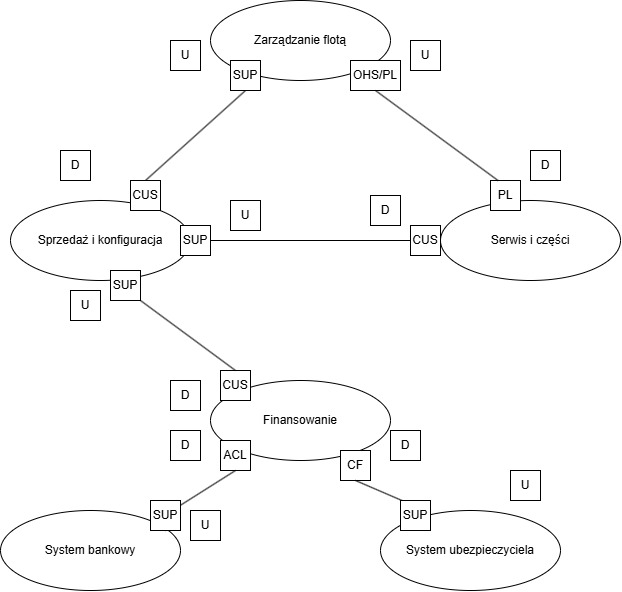
\includegraphics[width=0.8\textwidth]{media/ContextMapping.jpg}
%     \caption{Mapa kontekstów ograniczonych}
%     \label{fig:context-map}
% \end{figure}

% \begin{table}[H]
% \centering
% \caption{Mapowanie kontekstów}
% \label{tab:context-mapping}

% \renewcommand{\arraystretch}{1.2}
% \small

% \begin{tabular}{|p{3.2cm}|p{2.3cm}|p{2.3cm}|p{2.8cm}|p{4.2cm}|}
% \hline
% \textbf{Relacja} & \textbf{Upstream} & \textbf{Downstream} & \textbf{Wzorzec} & \textbf{Opis} \\
% \hline

% Flota $\rightarrow$ Sprzedaż &
% Flota &
% Sprzedaż &
% Customer-Supplier &
% Flota dostarcza dane o dostępności pojazdów dla sprzedaży. \\
% \hline

% Flota $\rightarrow$ Serwis &
% Flota &
% Serwis &
% Published Language &
% Flota publikuje zdarzenia logistyczne (VIN, status). \\
% \hline

% Sprzedaż $\rightarrow$ Serwis &
% Sprzedaż &
% Serwis &
% Customer-Supplier &
% Serwis przygotowuje pojazd zgodnie z zamówieniem. \\
% \hline

% Sprzedaż $\rightarrow$ Finansowanie &
% Sprzedaż &
% Finansowanie &
% Customer-Supplier &
% Finansowanie bazuje na danych z zamówienia. \\
% \hline

% Bank $\rightarrow$ Finansowanie &
% Bank &
% Finansowanie &
% ACL + Conformist &
% Finansowanie adaptuje zewnętrzny model banku przez ACL. \\
% \hline

% Ubezpieczyciel $\rightarrow$ Finansowanie &
% Ubezpieczyciel &
% Finansowanie &
% Conformist &
% System przyjmuje model ubezpieczyciela bez zmian. \\
% \hline

% \end{tabular}
% \end{table}